
The algorithm mapping multi-strand and multi-dimensional magnet geometries is explained in this section. Superconducting accelerator magnets are made from a strand or a bunch of strands, e.g. Rutherford cable\footnote{Rutherford cable is a type of an electrical cable used in superconducting technologies reducing Eddy current effects during the ramp up.}, wound multiple times in a certain pattern. Creating a CAD geometry where a~single strand domain is wound $n$ times would be a~complicated task. Therefore, every winding of the strand is considered as a~separate domain, as shown in Fig. \ref{fig:winding_geom_scheme}. The end of the windings marked in red are coupled with the neighbouring ones thermally and electrically, i.e. they are characterised by the same temperature and voltage. With such an approach, one can easily create multi-strand magnet geometries. Moreover, by specifying which windings are couple together, with the same numerical domain, one can also analyse magnets with different winding schemes.

\begin{figure}[H]
\centering
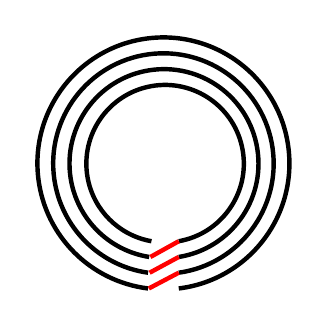
\begin{tikzpicture}[scale = 1]

\draw [ultra thick] (0,0) arc (-80:260:1);
\draw [ultra thick] (0,-0.2) arc (-81:261:1.2);
\draw [ultra thick] (0,-0.4) arc (-82:262:1.4);
\draw [ultra thick] (0,-0.6) arc (-83:263:1.6);

\draw [ultra thick, red] (0,0) -- (-0.36,-0.2);
\draw [ultra thick, red] (0,-0.2) -- (-0.37,-0.4);
\draw [ultra thick, red] (0,-0.4) -- (-0.38,-0.6);

\end{tikzpicture}
\caption{Domain representation with multiple windings.}
\label{fig:winding_geom_scheme}
\end{figure}

As illustrated in Fig.~\ref{fig: 3d_coil_illustation_with_2d_b_field}, a multi-strand domain is subjected to a varying magnetic field across the different windings~$i$. Since it is assumed that the coil is infinitely long, the magnetic field is calculated from a 2D model of a central magnet cross-section. 

\begin{figure}[H]
    \centering
    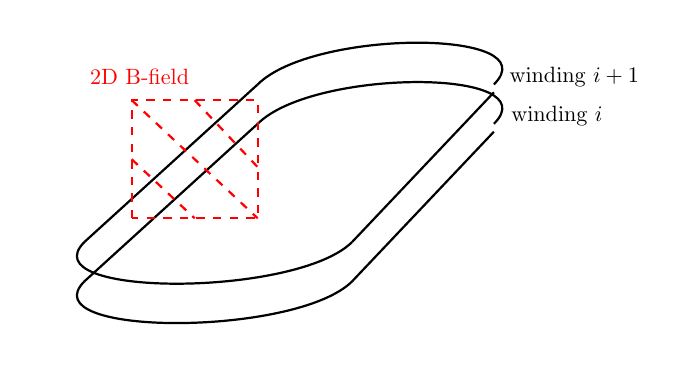
\begin{tikzpicture}[scale = 1]
        
        \foreach \y in {0,0.5} 
        \draw[thick,  black] (0.2,\y) -- (2,\y+1.9);
        
        \foreach \y in {0,0.5} 
        \draw[thick, black] (.2,\y) .. controls +(45:-1cm) and +(45:-1cm) .. (-3.2,\y);
        
        \foreach \y in {0,0.5} 
        \draw[thick,  black] (-3.2,\y) -- (-1,\y+2.0);
        
        \foreach \y in {0,0.5} 
        \draw[thick, black] (-1,\y+2) .. controls +(45:1cm) and +(45:1cm) .. (2,\y+2);
        
        \draw[thick, dashed, red] (-2.6,0.8) rectangle (-1.0,2.3);
        \draw[thick, dashed, red] (-2.6,1.55) -- (-1.8, 0.8);
        \draw[thick, dashed, red] (-2.6,2.3) -- (-1.0, 0.8);
        \draw[thick, dashed, red] (-1.8,2.3) -- (-1.0, 1.45);
        
        \node[scale = 0.8] at (2.8,2.1) {winding $i$};
        \node[scale = 0.8] at (3.02,2.6) {winding $i+1$};
        
        \node[red, scale = 0.8] at (-2.5,2.6) {2D B-field};
        
    \end{tikzpicture}
    \caption{Schematic of an assignment of a magnetic field to a multi-strand domain.}
    \label{fig: 3d_coil_illustation_with_2d_b_field}
\end{figure}

The different values of magnetic field are assigned to different windings, as shown in Fig.~\ref{fig:ansys_python_mapping scheme}. Since a different value of a magnetic field is assigned to each winding, every strand is characterised by different thermal and electrical material properties. Then, the multi-strand geometry is translated into a realistic one-dimensional cable with a length equal to the length of all the windings of a magnet. Each part of this coil length, $L_\text{coil, 1D}$ representing one winding is characterised by a different value of a magnetic field field~$B_\text{n}$.

\begin{figure}[H]
\centering
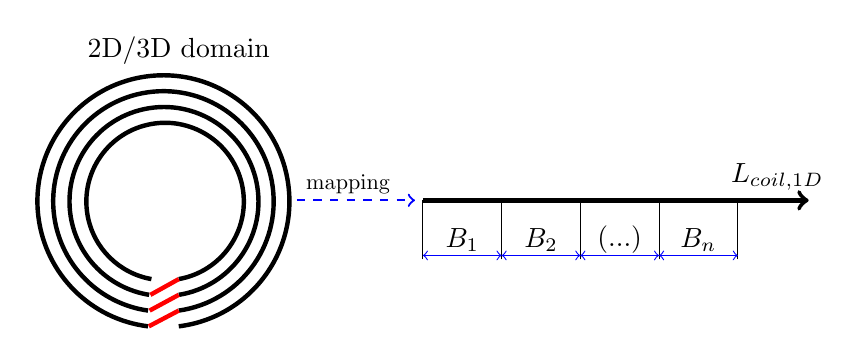
\begin{tikzpicture}[scale = 1]
\draw [ultra thick] (0,0) arc (-80:260:1);
\draw [ultra thick] (0,-0.2) arc (-81:261:1.2);
\draw [ultra thick] (0,-0.4) arc (-82:262:1.4);
\draw [ultra thick] (0,-0.6) arc (-83:263:1.6);
\draw [ultra thick, red] (0,0) -- (-0.36,-0.2);
\draw [ultra thick, red] (0,-0.2) -- (-0.37,-0.4);
\draw [ultra thick, red] (0,-0.4) -- (-0.38,-0.6);
\node[scale = 1.0] at (0,2.9) {2D/3D domain};
\draw [thick, dashed, blue, ->] (1.5,1) -- (3,1);
\node[scale = 0.8] at (2.15,1.2) {mapping};
\draw [ultra thick, ->] (3.1,1) -- (8,1);
\foreach \t in {3.1, 4.1, ..., 7.1}
\draw [thin] ({\t},0.25) -- ({\t},1);
\foreach \t in {3.1, 4.1, ..., 6.1}
\draw [thin, blue, <->] ({\t},0.3) -- ({\t+1},0.3);
\node[scale = 1.0] at (3.6,0.5) {$B_1$};
\node[scale = 1.0] at (4.6,0.5) {$B_2$};
\node[scale = 1.0] at (5.6,0.5) {(...)};
\node[scale = 1.0] at (6.6,0.5) {$B_\text{n}$};
\node[scale = 1.0] at (7.6,1.3) {$L_\text{coil, 1D}$};
\end{tikzpicture}
\caption{Multidimensional mapping scheme.}
\label{fig:ansys_python_mapping scheme}
\end{figure}

In Chapter~\ref{chapter: 1d_quench_propagation_modelling}, a uniform temperature was assumed in the cross-section of a strand which allowed for modelling the coil with a 1D longitudinal nodal domain. If such an assumption is not made, the composite strand is modelled with 2D or 3D nodal elements. As presented in Fig.~\ref{fig: mesh_generation_in_multidimensional_case}, the mesh is generated by specifying 2D nodal planes  uniformly distributed in a longitudinal direction of the coil. The planes are always perpendicular to the normal vector $\vec{n}$ of a directional spline. 

\begin{figure}[H]
    \centering
    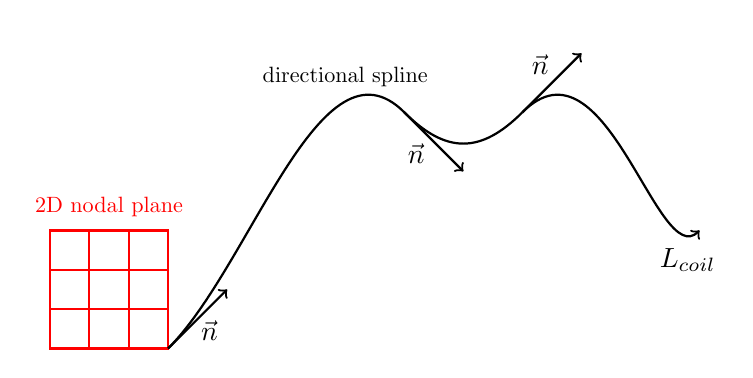
\begin{tikzpicture}[scale = 1.5]
        
        \draw[thick, red] (-1,1) rectangle (0,0);
        \draw[thick, red] (-1,1/3) -- (0,1/3);
        \draw[thick, red] (-1,2/3) -- (0,2/3);
        \draw[thick, red] (-1/3,0) -- (-1/3,1);
        \draw[thick, red] (-2/3,0) -- (-2/3,1);
        
        \draw[thick, black] (0,0) .. controls +(45:1cm) and +(135:1cm) .. (2,2);
        \draw[thick, black] (2,2) .. controls +(135:-0.5cm) and +(45:-0.5cm) .. (3,2);
        \draw[thick, black, ->] (3,2) .. controls +(45:1cm) and +(45:-0.5cm) .. (4.5,1);
        
        \draw[thick, black, ->] (0,0) -- (0.5,0.5);
        \draw[thick, black, ->] (2,2) -- (2.5,1.5);
        \draw[thick, black, ->] (3,2) -- (3.5,2.5);

        \node[red, scale=0.8] at (-0.5,1.2) {2D nodal plane};
        \node[black, scale=0.8] at (1.5,2.3) {directional spline};
        \node[black] at (0.35,0.15) {$\vec{n}$};
        \node[black] at (2.1,1.65) {$\vec{n}$};
        \node[black] at (3.15,2.4) {$\vec{n}$};
        \node[scale = 1.0] at (4.4,0.75) {$L_\text{coil}$};
        
    \end{tikzpicture}
    \caption{Multidimensional mesh generation in mapping algorithm.}
    \label{fig: mesh_generation_in_multidimensional_case}
\end{figure}

As illustrated in Fig.~\ref{fig:ansys_python_mapping scheme_nodes}, 2D nodal planes~$P_\text{n}$ are packed into a set of imaginary nodes~$N_\text{n}$ in the external routine calculating the propagation of quench. Each imaginary node~$P$ represents one plane~$N$. The position of the imaginary node~$N$ in space is an average position of all the nodes belonging to the plane~$P$. The creation of imaginary nodes serves for facilitating the assignment of quenched zones in time by an external routine. This process is performed in order to estimate the quench propagation only in the longitudinal direction.

\begin{figure}[H]
\centering
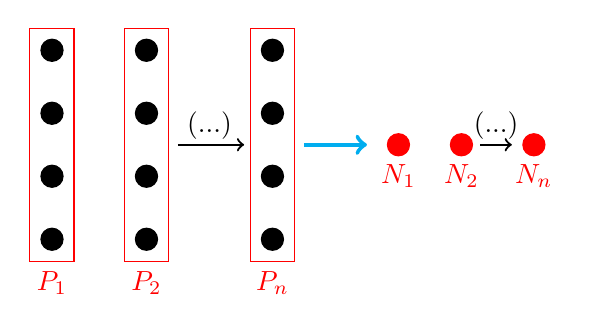
\begin{tikzpicture}[scale = 0.8]

    \foreach \t in {0,1,...,3}
    \filldraw[black] (0,{\t}) circle (5pt);
    \foreach \t in {0,1,...,3}
    \filldraw[black] (1.5,{\t}) circle (5pt);
    \foreach \t in {0,1,...,3}
    \filldraw[black] (3.5,{\t}) circle (5pt);
    \draw[red] (-0.35,-0.35) rectangle (0.35,3.35);
    \draw[red] (1.15,-0.35) rectangle (1.85,3.35);
    \draw[red] (3.15,-0.35) rectangle (3.85,3.35);
    \draw[thick,->] (2,1.5) -- (3.05,1.5);
    
    \node at (2.5, 1.8) {(...)};
    \node[red] at (0, -0.7) {$\text{P}_1$};
    \node[red] at (1.5, -0.7) {$\text{P}_2$};
    \node[red] at (3.5, -0.7) {$\text{P}_\text{n}$};
    
    \draw[ultra thick,->, cyan] (4,1.5) -- (5,1.5);
    \filldraw[red] (5.5,1.5) circle (5pt);
    \filldraw[red] (6.5,1.5) circle (5pt);
    \draw[thick,->] (6.8,1.5) -- (7.3,1.5);
    \filldraw[red] (7.65,1.5) circle (5pt);
    
    \node at (7.05, 1.8) {(...)};
    \node[red] at (5.5, 1) {$\text{N}_1$};
    \node[red] at (6.5, 1) {$\text{N}_2$};
    \node[red] at (7.65, 1) {$\text{N}_\text{n}$};

\end{tikzpicture}
\caption{Schematic of node assignment to imaginary nodes.}
    \label{fig:ansys_python_mapping scheme_nodes}
\end{figure}